\documentclass[a4paper,landscape,twocolumn]{article}
\usepackage[utf8]{inputenc}
\usepackage[LGR,T1]{fontenc}
\usepackage[ngerman,english]{babel}
\usepackage{amsmath}
\usepackage{amssymb}
\usepackage{amsfonts}
\usepackage{amsthm}
\usepackage{csquotes}
\usepackage{faktor}
\usepackage{fancyhdr}
\usepackage[margin=1in]{geometry}
\usepackage{imakeidx} % before hyperref
\usepackage[pdfborder={0 0 0},colorlinks=true,citecolor=red]{hyperref}
\usepackage{mathtools}
\usepackage{stmaryrd}
\usepackage{rotating}
\usepackage{bbold}

\title{Linear Algebra 2 -- Lecture Notes}
\author{Lukas Prokop}
\date{summer term 2016}

\newcommand\meta[3]{This #1 took place on #2 (#3).\par}
\newcommand\abs[1]{|\,#1\,|}
\newcommand\set[1]{\left\{#1\right\}}
\newcommand\setdef[2]{\left\{#1\,\middle|\,#2\right\}}
\newcommand\card[1]{\left|\,#1\,\right|}
\newcommand\divides[2]{#1\,\mid\,#2}
\newcommand\mathspace{\hspace{20pt}}
\newcommand\functional[1]{\left\langle{#1}\right\rangle}
\newcommand\Q{\mathbb{Q}}
\newcommand\nope{\lightning}
\newcommand\vecfour[4]{\begin{pmatrix} #1 \\ #2 \\ #3 \\ #4 \end{pmatrix}}
\newcommand{\textgreek}[1]{\begingroup\fontencoding{LGR}\selectfont#1\endgroup}

\newtheorem{theorem}{Theorem}
\newtheorem{defi}{Definition}
\newtheorem{ex}{Example}
\newtheorem{rem}{Remark}
\newtheorem{lemma}{Lemma}
\newtheorem{cor}{Corollary}

\DeclareMathOperator\Hom{Hom} % homomorphism
\DeclareMathOperator\End{End} % endomorphism
\DeclareMathOperator\Aut{Aut} % automorphism
\DeclareMathOperator\image{im} % image
\DeclareMathOperator\kernel{ker} % kernel
\DeclareMathOperator\rank{rank} % rank of a matrix

\DeclarePairedDelimiter\norm\lVert\rVert

\setcounter{MaxMatrixCols}{20}

\pagestyle{fancy}
\fancyhf{}
\chead{\Large{\textsc{Linear Algebra II -- Lecture Notes}}}
\lfoot{\makebox[\columnwidth]{\thepage}}
\rfoot{\makebox[\columnwidth]{\number\numexpr\value{page}+1}\stepcounter{page}}
\setlength{\headheight}{18pt}

\parindent0pt
\parskip5pt

\makeindex[name={German},title={German keywords}]
\makeindex[name={English},title={English keywords}]
\twocolumn

\begin{document}
\maketitle
\tableofcontents
\meta{lecture}{29th of Feb 2016}{Prof. Franz Lehner}

Exam: written and orally

Tutorial session:
\begin{itemize}
  \item Every Monday, 18:30-20:00, SR~11.34
  \item Contact: \href{mailto:gernot.holler@edu.uni-graz.at}{gernot.holler@edu.uni-graz.at}
\end{itemize}
Konversatorium:
\begin{itemize}
  \item Every Monday, 10:00--10:45, SR~11.33
\end{itemize}

Topics, wie already discussed:
\begin{itemize}
  \item Vector spaces
  \item Linear maps and their equivalence with matrices
  \item We introduced equivalence of matrices ($PAQ = B$)
  \item We defined the following techniques:
    \begin{itemize}
      \item Rank
      \item Linear equation system
      \item Inverse matrices
      \item Basis transformation
    \end{itemize}
\end{itemize}

In this semester, we will discuss:
\begin{itemize}
  \item
    $PAP^{-1}$, which is related to eigenvalues and diagonalization,
    hence $\bigvee_{P}^? PAP^{-1} = D$.
\end{itemize}

\clearpage
\section{Linear maps (cont.)}

\subsection[Addition to chapter 5.2.4]{Addition to chapter 5.2.4}

\index[English]{Dual space of a vector space}
\index[German]{\foreignlanguage{ngerman}{Dualraum des Vektorraums}}
\index[English]{Linear forms}
\index[German]{\foreignlanguage{ngerman}{Linearformen}}
\index[English]{Linear functionals}
\index[German]{\foreignlanguage{ngerman}{Lineare Funktionale}}
%
$\Hom(V,W)$ in special case $W = \mathbb K$. We define,
\[ V^* \coloneqq \Hom(V,\mathbb K) \]
also denoted $V'$ is called \emph{dual space} of vector space $V$.
The elements $v* \in V*$ is called \emph{linear forms} or \emph{linear functionals}.

We denote,
\[ v^*(v) \eqqcolon \functional{v*,v} \]

\subsection{Example}
\[ V = \mathbb K^n \]
$v^*: V \to \mathbb K$ is uniquely defined with values $v^*(e_i) \eqqcolon a_i$.
\[ \functional{v^*,v} = \functional{v^*, \sum_{i=1}^n v_i e_i} = \sum_{i=1}^n v_i \functional{v^*,e_i} \]
\[ \left(v^*\left(\sum_{i=1}^n v_i e_i\right) = \sum_{i=1}^n v_i v^*(e_i) = \sum_{i=1}^n a_i v_i\right) \]

\subsection{More general}
%
\index[English]{Dual basis of a vector space}
\index[German]{\foreignlanguage{ngerman}{Dualbasis eines Vektorraums}}
%
We know, $\dim{\Hom(V,W)} = \dim{V} \cdot \dim{W}$.
\begin{theorem}
  \label{5.26}
  Let $V$ be a vector space over $\mathbb K$.
  \begin{itemize}
    \item $\dim{V} \eqqcolon n < \infty \Rightarrow \dim{V^*} = n$ \\
      More precisely: Let $(b_1, \ldots, b_n)$ be a basis of $V$.
      Then \[
        b_k^*: b_i \mapsto \delta_{ik} = \begin{cases} 1 & i = k \\ 0 & \text{else} \end{cases}
      \]
      is a basis of $V^*$ and is called \emph{dual basis}.
    \item For $v^* \in V^*$ it holds that $v^* = \sum_{k=1}^n \functional{v^*, b_k} \cdot b_k^*$.
    \item If $\dim{V} = \infty, (b_i)_{i \in I}$ bass, then it holds that
      \[ (b^*_k)_{k \in I}, \functional{b_k^*, b_i} = \delta_{ik} \]
      is \emph{not} a basis of $V^*$.
  \end{itemize}
\end{theorem}
\begin{proof}
  \begin{itemize}
    \item Special case of 5.18 \\
      $(b^*_k)$ is linear independent, hence in $\sum_{i=1}^n \lambda_i b_i^* = 0$ all $\lambda_i = 0$.
      \[
        0 = \functional{\sum_{i=1}^n \lambda_i b_i^*, b_k}
          = \sum_{i=1}^n \lambda_i \functional{\underbrace{b_i^*, b_k}_{\delta_{ik}}}
          = \lambda_k \forall k
      \]
    \item Let $v \in V$ with $v = \sum_{i=1}^n v_i b_i$. We need to show
      \begin{align*}
        \functional{v^*, v} &\stackrel{!}{=} \functional{\sum_{k=1}^n \functional{v^*,b_w} b_n^*, v} \\
        \functional{\sum_{k=1}^n \functional{v^*, b_k} b_k^*, v}
            &= \sum_{k=1}^n \functional{v^*, b_k} \functional{b_k^*, v} \\
            &= \sum_{k=1}^n \functional{v^*, b_k} \functional{b_k^*, \sum_{i=1}^n v_i b_i} \\
            &= \sum_{k=1}^n \sum_{i=1}^n \functional{v^*, b_k} \underbrace{\functional{b_k^*, b_i}}_{\delta_{ki}} \cdot v_i \\
            &= \sum_{k=1}^n \functional{v^*, b_k} \functional{v^*, b_k} \cdot v_k \\
            &= \functional{v^*, \sum_{k=1}^n v_k b_k} \\
            &= \functional{v^*, v}
      \end{align*}
    \item (To be done in the practicals)
      Consider the functional
      \[ \functional{v^*, b_i} = 1 \Rightarrow v^* \not\in L((v_i^*)_{i \in I}) \]
  \end{itemize}
\end{proof}

\subsection{Remark and a definition for bilinearity}
\index[English]{Bilinear map}
\index[German]{\foreignlanguage{ngerman}{Bilineare Abbildung}}
\index[English]{Multilinear map}
\index[German]{\foreignlanguage{ngerman}{Multilineare Abbildung}}
%
The mapping $V^* \times V \to \mathbb K$ is linear in $v$ (with fixed $v^*$)
with $(v^*, v) \mapsto \functional{v^*, v}$ is linear in $v^*$ (with fixed $v$).
Such a mapping is called \emph{bilinear}.

A mapping $F: V_1 \times \ldots \times V_n \to W$ is called \emph{multilinear} ($n$-linear)
if it is linear in every component. Formally:
\[
  F(v_1, \ldots, v_{k-1}, \lambda v'_k + \mu v''_k, v_{k+1}, \ldots, v_n)
\] \[
    = \lambda F(v_1, \ldots, v_{k-1}, v'_k, v_{k+1}, \ldots, v_n) + \mu F(v_1, \ldots, v''_k, v_{k+1}, \ldots, v_n)
\]

\subsection{Example}
\label{ex-5.28}
%
\[ V = \mathbb K[x] \text{ polynomials} \]
Basis: $\setdef{x^k}{k \in \mathbb N_0}$ and $\dim{V} = \aleph_0$

Every $v^* \in V^*$ is uniquely defined by $a_k \coloneqq \functional{v^*, x^k}$
\[ (a_k)_{k \in \mathbb N_0} \]
$V^* \cong \mathbb K[[t]]$ are the formal power series
\[ = \setdef{\sum_{k=0}^\infty a_k t^k}{a_k \in \mathbb K} \]
\[ \lambda \sum_{k=0}^\infty a_k t^k + \mu \sum_{k=0}^\infty b_k t^k = \sum_{k=0}^\infty (\lambda a_k + \mu b_k) t^k \]
(Compare with Taylor series $f(x) = \sum_{n=0}^\infty \frac{f^{(n)}(0)}{n!} x^n)$)
\[ \functional{\sum_{k=0}^\infty a_k t^k, \sum_{k=0}^n b_k x^k} \eqqcolon \sum_{k=0}^n a_k b_k \text{ is well-defined} \]
\[ \rightarrow \mathbb K[x]^* \cong \mathbb K[[t]] \]

\subsection{Example}
\label{ex-5.29}
\[ C[0,1] \text{ continuous functions} \]
Example:
\begin{ex}
\[ x \in [0,1] \qquad \delta_{x}: C[0,1] \to \mathbb R \]
\[ f \mapsto f(x) \]
\[ \functional{\delta_x, f} = f(x) \]
\[ \functional{\delta_x, f} = f(x) \]
\[ I(f) = \int_0^1 f(x) \, \text{d}x \text{ is linear} \]
\end{ex}

\[ \functional{I_g,f} = \int_0^1 f(x) g(x) \, \text{d}x \]
\[ g \in C[0,1] \text{ is fixed} \]
\[ \Rightarrow I_g \in C[0,1] \]
\[
  \functional{I_g, \lambda f_1 + \mu f_2}' = \int_0^1 (\lambda f_1(x) + \mu f_2(x)) g(x) \,\text{d}x
\] \[
  = \lambda \int_0^1 f_1(x) g(x) \,\text{d}x + \mu \int_0^1 f_2(x) g(x) \,\text{d}x
\]
This also works with non-continuous $g$ (it suffices to have $g$ integratable). (Compare with measure theory and Riesz' theorem)

Does there exist some $g$ such that $f(x) = \functional{\delta_x, f} = \int_0^1 f(t) g(t) \,\text{d}t$.
(Compare with Dirac's $\delta$ function and Schwartz/Sobder theory)

\[ V^{**} = \left(V^*\right)^* \cong V \text{ if } \dim{V} < \infty \]

\begin{lemma}
  \label{lemma-5.30}
  Let $V$ be a vector space over $\mathbb K$. It requires that $\dim{V} < \infty$ and the Axiom of Choice holds.
  \begin{itemize}
    \item $v \in V \setminus \set{0} \Leftrightarrow \bigvee_{v^* \in V^*} \functional{v^*,v} \neq 0$
    \item $\bigwedge_{v \in V} v = 0 \Leftrightarrow \bigwedge_{v^* \in V^*} \functional{v^*,v} = 0$
  \end{itemize}
\end{lemma}
\begin{proof}
  Addition $v$ to a basis $B$ of $V$:
  Define $v^* \in V^*$ by
  \[ \functional{v^*,b} = \begin{cases} 1 & b = v \\ 0 & b \neq v \end{cases} \text{ for } b \in B \]
\end{proof}

\index[English]{Bidual space}
\index[German]{\foreignlanguage{ngerman}{Bidualraum}}
\begin{theorem}
  \label{theorem-5.31}
  Let $V$ be a vector space over $\mathbb K$.
  \begin{itemize}
    \item The map $\iota: V \to V^{**} \coloneqq (V^*)^*$ is called \emph{bidual space}.
      \[ \functional{\iota(v), v^*} \coloneqq \functional{v^*,v} \]
      is linear and injective.
    \item if $\dim{V} < \infty$, then isomorphism.
  \end{itemize}
\end{theorem}
\begin{proof}
  \begin{itemize}
    \item Linearity
      \[ \iota(\lambda v + \mu w) \stackrel{!}{=} \lambda \iota(v) + \mu \iota (w) \]
      must hold in every point $v^* \in V^*$:
      \begin{align*}
        \functional{\iota(\lambda v + \mu w), v^*}
          &= \functional{v^*, \lambda v + \mu w} \\
          &= \lambda \functional{v^*,v} + \mu \functional{v^*, w} \\
          &= \lambda \functional{\iota(v), v^*} + \mu \functional{\iota(w), v^*} \\
          &= \functional{\lambda \iota(v) + \mu \iota(w), v^*}
      \end{align*}
      Is it injective?
      Let $v \in \kernel{\iota}$.
      \[ \functional{\iota(v), v^*} = 0 \quad \forall v^* \in V^* \]
      \[ \Rightarrow \functional{v^*,v} = 0 \quad \forall v^* \in V^* \]
      \[ \xRightarrow{\text{Lemma~\ref{lemma-5.30}}} v = 0 \]
    \item Follows immediately, because the dimension is equal.
  \end{itemize}
\end{proof}

\index[English]{Transposed map}
\index[German]{\foreignlanguage{ngerman}{Transponierte Abbildung}}
\begin{defi}
  \label{defi-5.32}
  Let $V,W$ be vector spaces over $\mathbb K$. $f \in \Hom(V,W)$.
  We define $f^T \in \Hom(W^*,V^*)$ using $f^T(w^*) \in V^*$ via
  \[ \functional{f^T(w^*),v} = \functional{w^*,f(v)} = w^*(f(v)) = w^* \circ f(v) \]
  \[ f^T(w^*) = w^* \circ f \text{ is linear} \Rightarrow f^T(w^*) \in V^* \]
  $V$ to $W$ (with $f$) and $W$ to $\mathbb K$ (with $w^*$).

  $f^T$ is called \emph{transposed map}.
\end{defi}

\begin{ex}
  (See practicals)
  Let $\dim{V} = n$ and $\dim{W} = m$ with $B \subseteq V$ and $C \subseteq W$ as bases
  and dual bases $B^* \subseteq V^*$ and $C^* \subseteq W^*$
  \[ \Phi_{B^*}^{C^*}(f^T) = \Phi_C^B(f)^T \quad\text{transposition of matrices} \]
\end{ex}

\meta{lecture}{2nd of March 2016}{Franz Lehner}

\section{Determinants}
%
Leibnitz~1693 ($3\times 3$ matrices) \\
Seki Takukazu~1685 (most general version) \\
Gauß~1801 (\enquote{determinant}) \\
Cayley~1845 (on matrices)

\begin{description}
  \item[$n=2$]
    \begin{align*}
      ax + by &= e \\
      cx + dy &= f
    \end{align*}
    \[
      \begin{array}{cc|c}
        a & b & e \\
        c & d & f
      \end{array}
    \]
    \begin{enumerate}
      \item Case 1: $a \neq 0$ (multiply first row $-\frac{a}{b}$ times second row)
        \[
          \begin{array}{cc}
            a & b \\
            c & d \\
          \hline
            a & b \\
            0 & d - \frac{bc}{a}
          \end{array}
        \]
        Unique solution:
        \[ d - \frac{bc}{a} \neq 0 \]

      \item Case 2: $c \neq 0$ (multiple second row $-\frac{a}{c}$ times first row)
        \[
          \begin{array}{cc}
            a & b \\
            c & d \\
          \hline
            0 & b-\frac{ad}{c} \\
            c & d
          \end{array}
        \]
        Unique solution:
        \[ b - \frac{ad}{c} \neq 0 \]
    \end{enumerate}

    This gives us
    \[ ad - bc \neq 0 \]
\end{description}

\index[English]{Determinant}
\index[German]{\foreignlanguage{ngerman}{Determinante}}
\begin{defi}
  \[ \det\begin{pmatrix} a & b \\ c & d \end{pmatrix} = ad - bc = \begin{vmatrix} a & b \\ c & d \end{vmatrix} \]
  is called \emph{determinant} of $\begin{pmatrix} a & b \\ c & d \end{pmatrix}$.
\end{defi}

\subsection{Properties of determinants}
%
\begin{itemize}
  \item The determinant is bilinear in the columns and rows.

    \[ A = \begin{pmatrix} a & b \\ c & d \end{pmatrix} = (v,w) \]
    where $v$ and $w$ are column vectors of $A$.
    \[ \det(\lambda v_1 + \mu v_2, w) = \lambda \det(v_1, w) + \mu \det(v_2, w) \]
    \[ \det(v, \lambda w + \mu w_2) = \lambda \det(v, w_1) + \mu \det(v, w_2) \]

    \[
      \det(\lambda v_1 + \mu v_2, w) =
      \begin{vmatrix}
        \lambda a_1 + \mu a_2 & b \\
        \lambda c_1 + \mu c_2 & d
      \end{vmatrix}
    \] \[
      = (\lambda a_1 + \mu a_2) d - (\lambda c_1 + \mu c_2) b
    \] \[
      = \lambda (a_1 d - c_1 b) + \mu (a_2 d - c_2 b)
    \] \[
      = \lambda \begin{vmatrix} a_1 & b \\ c_1 & d \end{vmatrix}
      + \mu \begin{vmatrix} a_2 & b \\ c_2 & d \end{vmatrix}
    \]
    \[ \begin{vmatrix} a & b \\ c & d \end{vmatrix} = \begin{vmatrix} a & c \\ b & d \end{vmatrix} \]
  \item
    $\det(v,v) = 0$.
    \[ \begin{vmatrix} a & a \\ c & c \end{vmatrix} = ac - ac = 0 \]
  \item
    \[ \det\begin{pmatrix} 1 & 0 \\ 0 & 1 \end{pmatrix} = \det(e_1, e_2) = 1 \]
\end{itemize}

\begin{theorem}
  \label{satz-7.3}
  The properties 1--3 of determinants (see above) characterize the determinant.

  Let $\varphi: \mathbb K^2 \times \mathbb K^2 \to \mathbb K$
  \begin{itemize}
    \item bilinear
    \item $\bigwedge_{v \in \mathbb K^2} \varphi(v,v) = 0$
    \item $\varphi(e_1, e_2) = 1$.
      Then it holds that $\varphi = \det$.
  \end{itemize}
\end{theorem}
\begin{proof}
  To show: $\varphi(v,w) = \det(v,w) \forall v,w \in \mathbb K^2$

  \[
    v = \underbrace{a e_1 + c e_2}_{\begin{pmatrix} a \\ c \end{pmatrix}}
    \qquad
    w = \underbrace{b e_1 + d e_2}_{\begin{pmatrix} b \\ d \end{pmatrix}}
  \] \begin{align*}
    \varphi(v,w) &= \varphi(a e_1 + c e_2, b e_1 + d e_2) \\
      &= a\varphi(e_1, be_1 + de_2) + c \cdot \varphi(e_2, be_1 + de_2) \\
      &= ad \underbrace{\varphi(e_1, e_2)}_{=1} + \underbrace{ab \varphi(e_1, e_1)}_{=0} + cb \varphi(e_2, e_1) + cd \underbrace{\varphi(e_2, e_2)}_{=0}
  \end{align*}
\end{proof}

\begin{lemma}
  \label{lemma-7.4}
  From (i) bilinearity and (ii) $\bigwedge_{v \in \mathbb K^2} \varphi(v,v) = 0$ it follows that
  \[ \bigwedge_{v,w \in \mathbb K^2} \varphi(v,w) = - \varphi(w, v) \]

  \begin{align*}
    0 \overset{\text{(ii)}}{=} \varphi(v+w, v+w)
      &\overset{\text{(i)}}{=} \varphi(v,v) + \varphi(v,w) + \varphi(w,v) + \varphi(w,w) \\
      &\overset{\text{(ii)}}{=} \varphi(v,w) + \varphi(w,v)
  \end{align*}
\end{lemma}

\subsection{Geometric interpretation of the determinant}
%
Consider an area with $w$ defining its breath and $v$ its depth (hence the area spanning vectors).
Let $e_1$ and $e_2$ be the spanning vectors of a rectangle corresponding to the parallelogram.
$\det(v,w)$ is the surface of the spanned parallelogram.
The sign defines the orientation of the pair $(v, w)$.
\[ \det(e_1, e_2) = 1 \qquad \det(e_2, e_1) = -1 \]

There are surfaces where the surface is infinite if you follow a vector in some direction:
\begin{itemize}
  \item Möbius strip
  \item Klein's bottle (named after Felix~Klein)
\end{itemize}

\[ A = \abs{v} \cdot h \]

\begin{figure}[!h]
  \begin{center}
    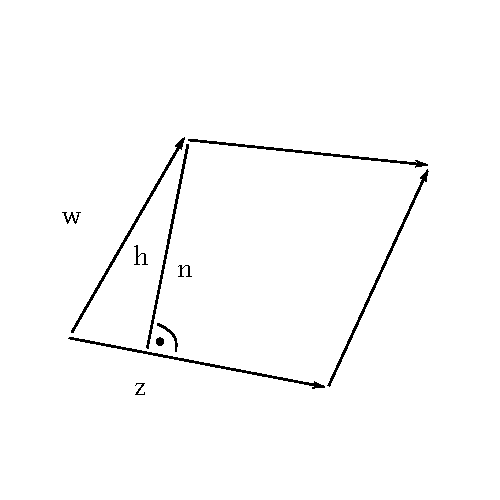
\includegraphics{img/parallelogram.pdf}
    \caption{Parallelogram}
    \label{img:para}
  \end{center}
\end{figure}

Consider Figure~\ref{img:para}.
$h$ is the length of the projection of $w$ to $v^\bot$.
\[
  v = \begin{pmatrix} a \\ b \end{pmatrix}
  \to
  \vec{n} = \begin{pmatrix} -b \\ a \end{pmatrix}
\] \[
  \langle \begin{pmatrix} c \\ d \end{pmatrix}, \begin{pmatrix} -b \\ a \end{pmatrix} \rangle
  = ad - bc
\]

\begin{proof}[Second proof]
  $A(v,w)$ satisfies properties (i)---(iii).
  \begin{itemize}
    \item Property (iii) follows immediately (the area of unit vectors in two dimensions is 1).
    \item Property (ii) follows immediately (the area of two vectors in the same direction is 0).
  \end{itemize}
  Property (i) defines the linearity in $v$
  \begin{enumerate}
    \item If $v,w$ are linear dependent, then $A(v,w) = 0$ (one is a multiple of the other)
    \item $n\in \mathbb N$ with $A(nv,w) = nA(v,w)$
    \item For $\tilde{v} = n \cdot v$:
      \[ A(\tilde{v}, w) = n \cdot A(\frac{\tilde{v}}{n}, w) \]
      \[ \Rightarrow A(\frac{\tilde{v}}{n}, w) = \frac1n A(\tilde{v}, w) \]
      \begin{align*}
        A(nv,w) &= n A(v,w) \\
        A(\frac1n v, w) &= \frac1n A(v,w) \\
        A(\frac mn v, w) &= \frac mn A(v,w) \\
        A(-v,w) &= -A(v,w)
      \end{align*}
      From continuity it follows that $A(\lambda u, w) = \lambda A(v, w)$ for $\lambda \in \mathbb R$.
      Analogously $A(v, \lambda w) = \lambda A(v, w)$.
    \item The sum is given with
      \[ A(v + w, w) = A(v, w) \]
      Compare with Figure~\ref{img:pt}, where $\operatorname{area}(2) + \operatorname{area}(3) = \operatorname{area}(2) + \operatorname{area}(1)$.
      \begin{figure}[!h]
        \begin{center}
          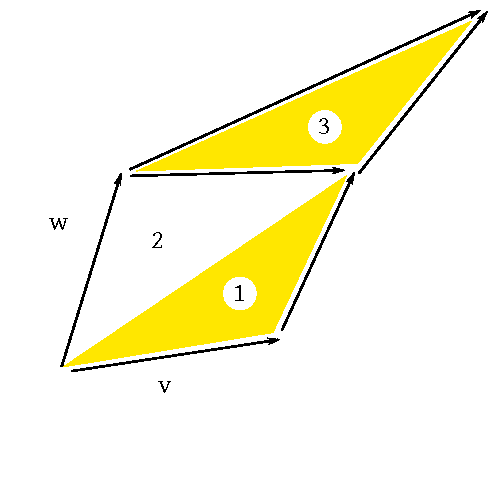
\includegraphics{img/parallelogram-translation.pdf}
          \caption{Translation of area 1 to area 3.}
          \label{img:pt}
        \end{center}
      \end{figure}
      \begin{align*}
        A(\lambda v + \mu w, w)
          &= A(\lambda v + \mu w, \frac{1}{\mu} \mu w) \\
          &= \frac1\mu A(\lambda v + \mu w, \mu w) \\
          &= \frac{1}{\mu} A(\lambda v, \mu w) \\
          &= A(\lambda v, w)
      \end{align*}

      General case: $v, w$ are linear independent and therefore basis of $\mathbb R^2$.
      Besides that, $v_1$ and $v_2$ are arbitrary.
      \begin{align*}
        v_1 &= \lambda_1 v + \mu_1 w \\
        v_2 &= \lambda_2 v + \mu_2 w
      \end{align*}
      \begin{align*}
        A(v_1 + v_2, w)
          &= A(\lambda_1 v + \mu_1 w + \lambda_2 v + \mu_2 w, w) \\
          &= A((\lambda_1 + \lambda_2) v + (\mu_1 + \mu_2) w, w) \\
          &= A((\lambda_1 + \lambda_2) v, w) \\
          &= (\lambda_1 + \lambda_2) A(v, w) \\
          &= A(\lambda_1 v, w) + A(\lambda_2 v, w)
      \end{align*}
      \[ A(\lambda_1 v + \mu_1 w, w) + A(\lambda_2 v + \mu_2 w, w) = A(v_1, w) + A(v_2, w) \]
      Additivity follows.
  \end{enumerate}
\end{proof}

\index[English]{determinant form}
\index[German]{\foreignlanguage{ngerman}{Determinantenform}}
\index[English]{Multilinearity}
\index[German]{\foreignlanguage{ngerman}{Multilinearität}}
\begin{defi}
  Let $\dim{V} = n$. A \emph{determinant form} is a map
  \[ \triangle: V^n \to \mathbb K \]
  with properties:
  \begin{enumerate}
    \item
      \[
        \bigwedge_{\lambda} \bigwedge_{k} \bigwedge_{a_1,\ldots,a_n \in V}
        \triangle (a_1, \ldots, a_{k-1}, \lambda a_k, a_{k+1}, \ldots, a_n)
        = \lambda \triangle (a_1, \ldots, a_k, \ldots, a_n)
      \]
    \item
      \[
        \bigwedge_k \bigwedge_{\substack{a_1, \ldots, a_n \\ a'_k, a''_k}}
        \triangle(a_1, \ldots, a_{k-1}, a'_k + a''_k, a_{k+1}, \ldots, a_n)
      \] \[
        \coloneqq \triangle(a_1, \ldots, a_{k-1}, a'_k + a''_k, a_{k+1}, \ldots, a_n)
      \]
    \item
      \[ \triangle(a_1, \ldots, a_n) = 0 \]
      if $\bigvee_{k \neq l} a_k = e_l$
      if $\triangle \neq 0$, i.e. $\triangle$ is non-trivial.
  \end{enumerate}
  Multilinearity is defined by the first two properties.
  Multilinearity means linearity in $a_k$ if $a_1, \ldots, a_{k-1}, a_{k+1}, \ldots, a_n$
  get fixed.
\end{defi}

\begin{theorem}
  \[ \dim{V} = n \]
  \[ \triangle: V^n \to \mathbb K \text{ is determinant form} \]
  Then,
  \begin{enumerate}
    \item[4.]
      \[
        \bigwedge_{\lambda \in \mathbb K} \bigwedge_{i \neq j}
        \triangle(a_1, \ldots, a_{i-1}, a_{i} + \lambda a_j, a_{i+1}, \ldots, a_n)
        = \triangle(a_1, \ldots, a_i, \ldots, a_n)
      \]
      \enquote{Addition of $\lambda a_j$ to $a_i$ does not change $\triangle$}
    \item[5.]
      \[
        \bigwedge_{i>j} \triangle(a_1, \ldots, a_{j-1}, a_i, a_{j+1}, \ldots, a_{i-1}, a_j, a_{i+1}, \ldots, a_n)
      \] \[
        = -\triangle (a_1, \ldots, a_j, \ldots, a_i, \ldots, a_n)
      \]
      \enquote{Exchanging $a_i$ with $a_j$ inverts the sign}
  \end{enumerate}
\end{theorem}
\begin{proof}
  \begin{enumerate}
    \item[4.]
      \[
        \triangle(a_1, \ldots, a_i + \lambda a_j, \ldots, a_n)
      \]
      Without loss of generality: $i < j$.
      From properties 1 and 2 it follows that:
      \[
        = \triangle (a_1, \ldots, a_i, a_j, a_n)
        + \lambda \triangle(a_1, \ldots, a_j, a_j, \ldots, a_k)
      \]
      Oh, $a_j$ occurs twice! Once at index $i$ and once at index $j$.
      \[ = 0 \]
      due to property 3.
    \item[5.]
      \begin{align*}
        0 &\stackrel{\text{property~3}}= \triangle (a_1, \ldots, a_{i-1}, a_i + a_j, \ldots, a_{j-1}, a_i + a_j, \ldots, a_n) \\
          &= \triangle(a_1, \ldots, a_{i-1}, \mathbf{a_i}, \ldots, a_{j-1}, \mathbf{a_i}, \ldots, a_n) \mathbf{= 0} \\
          &+ \triangle(a_1, \ldots, a_{i-1}, \mathbf{a_i}, \ldots, a_{j-1}, \mathbf{a_j}, \ldots, a_n) \\
          &+ \triangle(a_1, \ldots, a_{i-1}, \mathbf{a_j}, \ldots, a_{j-1}, \mathbf{a_i}, \ldots, a_n) \\
          &+ \triangle(a_1, \ldots, a_{i-1}, \mathbf{a_j}, \ldots, a_{j-1}, \mathbf{a_j}, \ldots, a_n) \mathbf{= 0} \\
          &\Rightarrow \delta
      \end{align*}
  \end{enumerate}
\end{proof}

\begin{defi}
  \label{defi-7.8}
  A permutation of order $n$ is a bijective mapping $\pi: \set{1, \ldots, n} \to \set{1, \ldots, n}$.
  \[ \sigma_n = \text{ set of all permutations} \]
\end{defi}
\begin{rem}
  Notation:
  We write the elements in the first row and their images in the second row.
\end{rem}
\begin{defi}
  \label{defi-7.9}
  $\sigma_n$ constitutes (in terms of composition) a group with neutral element $\text{id}$,
  the so-called symmetric group.
\end{defi}

In the previous course (Theorem~1.40) we hvae proven: Compositions of bijective functions are bijective.
\begin{rem}
  For $n \geq 3$, $\sigma_n$ is non-commutative
\end{rem}
\begin{theorem}
  \label{satz-7.10}
  \[ \card{\sigma_n} = n! \]
\end{theorem}
\begin{rem}
  These are \enquote{a lot}!
\end{rem}
\begin{ex}
  \label{example-7.11}
  \[
    \begin{pmatrix}
      1 & 2 & 3 & 4 \\
      4 & 1 & 3 & 2
    \end{pmatrix} \circ \begin{pmatrix}
      1 & 2 & 3 & 4 \\
      1 & 3 & 4 & 2
    \end{pmatrix}
    = \begin{pmatrix}
      1 & 2 & 3 & 4 \\
      4 & 3 & 2 & 1
    \end{pmatrix}
  \] \[
    \begin{pmatrix}
      1 & 2 & 3 & 4 \\
      4 & 1 & 3 & 2
    \end{pmatrix}^{-1}
    = \begin{pmatrix}
      1 & 2 & 3 & 4 \\
      2 & 4 & 3 & 1
    \end{pmatrix}
  \]
\end{ex}

\index[English]{transposition}
\index[German]{\foreignlanguage{ngerman}{Vertauschung}}
\begin{defi}
  A \emph{transposition} is a permutation of the structure
  \[
    \tau = \tau_{ij}:
    \begin{array}{c}
      i \mapsto j \\
      j \mapsto i \\
      k \mapsto h
    \end{array}
    \text{ if } k \notin \set{i,j}
  \]
  Then $\tau_{ij}^{-1} = \tau_{ij}$, hence $\tau_{ij}^2 = \text{id}$.
\end{defi}
\begin{theorem}
  \label{theorem-7.13}
  $\sigma_n$ is generated by transpositions.
  With other words, every permutation $\pi$ can be represented as composition of transpositions
  \[ \pi = \tau_1 \circ \ldots \circ \tau_k \]
\end{theorem}
\begin{proof}
  \[
    \pi = \begin{pmatrix}
      1 & 2 & \ldots & n \\
      \pi(1) & \pi(2) & \ldots & \pi(n)
    \end{pmatrix}
  \]
  If $\pi = \text{id}$,
  \[ \pi = \pi \quad \tau \coloneqq \text{id} \]
  If $\pi \neq \text{id}$,
  \[ k_1 = \min\setdef{k}{k \neq \pi(k)} \]
  \begin{enumerate}
    \item
      \[ \tau_1 = \tau_{k_1 \pi(k_1)} \]
      \[
        \pi_1 = \tau_1 \circ \pi =
        \begin{pmatrix}
          1 & \ldots & \substack{k-1 \\ 1} & k_1 & \ldots \\
          1 & \ldots & \substack{k-1 \\ 1} & k_1 & \ldots
        \end{pmatrix}
      \]
      Example:
      Consider $\begin{pmatrix}
        1 & 2 & 3 & 4 & 5 & 6 & 7 \\
        1 & 3 & 5 & 4 & 7 & 6 & 2
      \end{pmatrix}$.
      \[ k_1 = 2 \]
      \[ \tau_1 = \tau_{23} \]
      \[
        \pi_1 = \tau_1 \circ \pi =
        \begin{pmatrix}
          1 & 2 & 3 & 4 & 5 & 6 & 7 \\
          1 & 2 & 5 & 4 & 7 & 6 & 3
        \end{pmatrix}
      \]
    \item
      \[ k_2 = \min\setdef{k}{k \neq \pi_1(k)} > k_1 \]
      \[ \tau_2 = \tau_{k_2,\pi(k_2)} \]
      And so on and so forth. $k_j > k_{j-1}$ ends after $\leq n$ steps.
      \[ \tau_k \circ \tau_{k-1} \circ \ldots \circ \tau_1 \circ \pi = \text{id} \]
      \[ \Rightarrow \pi = \tau_1 \circ \tau_2 \circ \ldots \circ \tau_k \]

      Regarding the example:
      \[ k_2 = 3 \]
      \[ \tau_2 = \tau_{35} \]
      \[
        \pi_2 = \tau_2 \circ \pi_1 = \tau_2 \circ \tau_1 \circ \pi =
        \begin{pmatrix}
          1 & 2 & 3 & 4 & 5 & 6 & 7 \\
          1 & 2 & 3 & 4 & 7 & 6 & 5
        \end{pmatrix}
      \]
      \[ k_3 = 5 \quad \tau_3 = \tau_{57} \]
      \[ \Rightarrow \pi = \tau_{23} \circ \tau_{35} \circ \tau_{57} \]
  \end{enumerate}
\end{proof}

\index[English]{Malposition}
\index[German]{\foreignlanguage{ngerman}{Fehlstand (Permutation)}}
\begin{defi}
  \label{def-7.14}
  A \emph{malposition} of $\pi$ is a pair $(i,j)$ such that
  $i < j$ with $\pi(i) > \pi(j)$.
  Let $F_\pi$ be the set of malpositions of $\pi$.
  \[ f_{\pi} \coloneqq \card{F_\pi} \]
  \[ \operatorname{sign}(\pi) \coloneqq (-1)^{f_\pi} \eqqcolon (-1)^\pi \]
\end{defi}

\begin{ex}
  \label{example-7.15}
  \[
    \pi = \begin{pmatrix}
      1 & 2 & 3 & 4 & 5 & 6 & 7 \\
      1 & 3 & 5 & 4 & 7 & 6 & 2
    \end{pmatrix}
  \] \[
    F_\pi = \set{(2,7), (3,4), (3,7), (4,7), (5,6), (5,7), (6,7)}
  \]
  \[ f_\pi = 7 \qquad \operatorname{sign}(\pi) = -1 \]
\end{ex}

\clearpage
\begin{otherlanguage}{ngerman}
\printindex[German]
\end{otherlanguage}
\printindex[English]

\end{document}
